% "Training in simulation" figure for the A1 poster. Compile on its own, then in the poster:
%   \includegraphics[width=\linewidth]{images/fig_training_poster.pdf}
\documentclass[12pt, border=4pt]{standalone}
\usepackage{tikz}
\usetikzlibrary{arrows.meta,positioning,calc,fit,backgrounds,shadings,shapes.geometric}
\renewcommand{\familydefault}{\sfdefault}

\definecolor{saclaydk}{RGB}{27,67,32}
\definecolor{mandarine}{RGB}{243,115,32}
\definecolor{vert}{RGB}{140,198,62}
\definecolor{bleu}{RGB}{80,144,205}
\definecolor{rouge}{RGB}{198,11,70}

\tikzset{
  box/.style={rounded corners=4pt, line width=1.4pt, align=center, inner sep=5pt},
  hw/.style={box, draw=saclaydk, fill=vert!18},
  nn/.style={box, draw=mandarine, fill=mandarine!18, line width=2pt},
  chip/.style={rounded corners=3pt, draw=saclaydk!70, fill=white, line width=0.8pt,
               font=\normalsize, minimum width=4.7cm, inner sep=3pt},
  arr/.style={-{Stealth[length=4mm,width=3mm]}, line width=2pt, draw=saclaydk!80},
  arrb/.style={arr, draw=bleu},
  arrnn/.style={arr, draw=mandarine},
}

\begin{document}
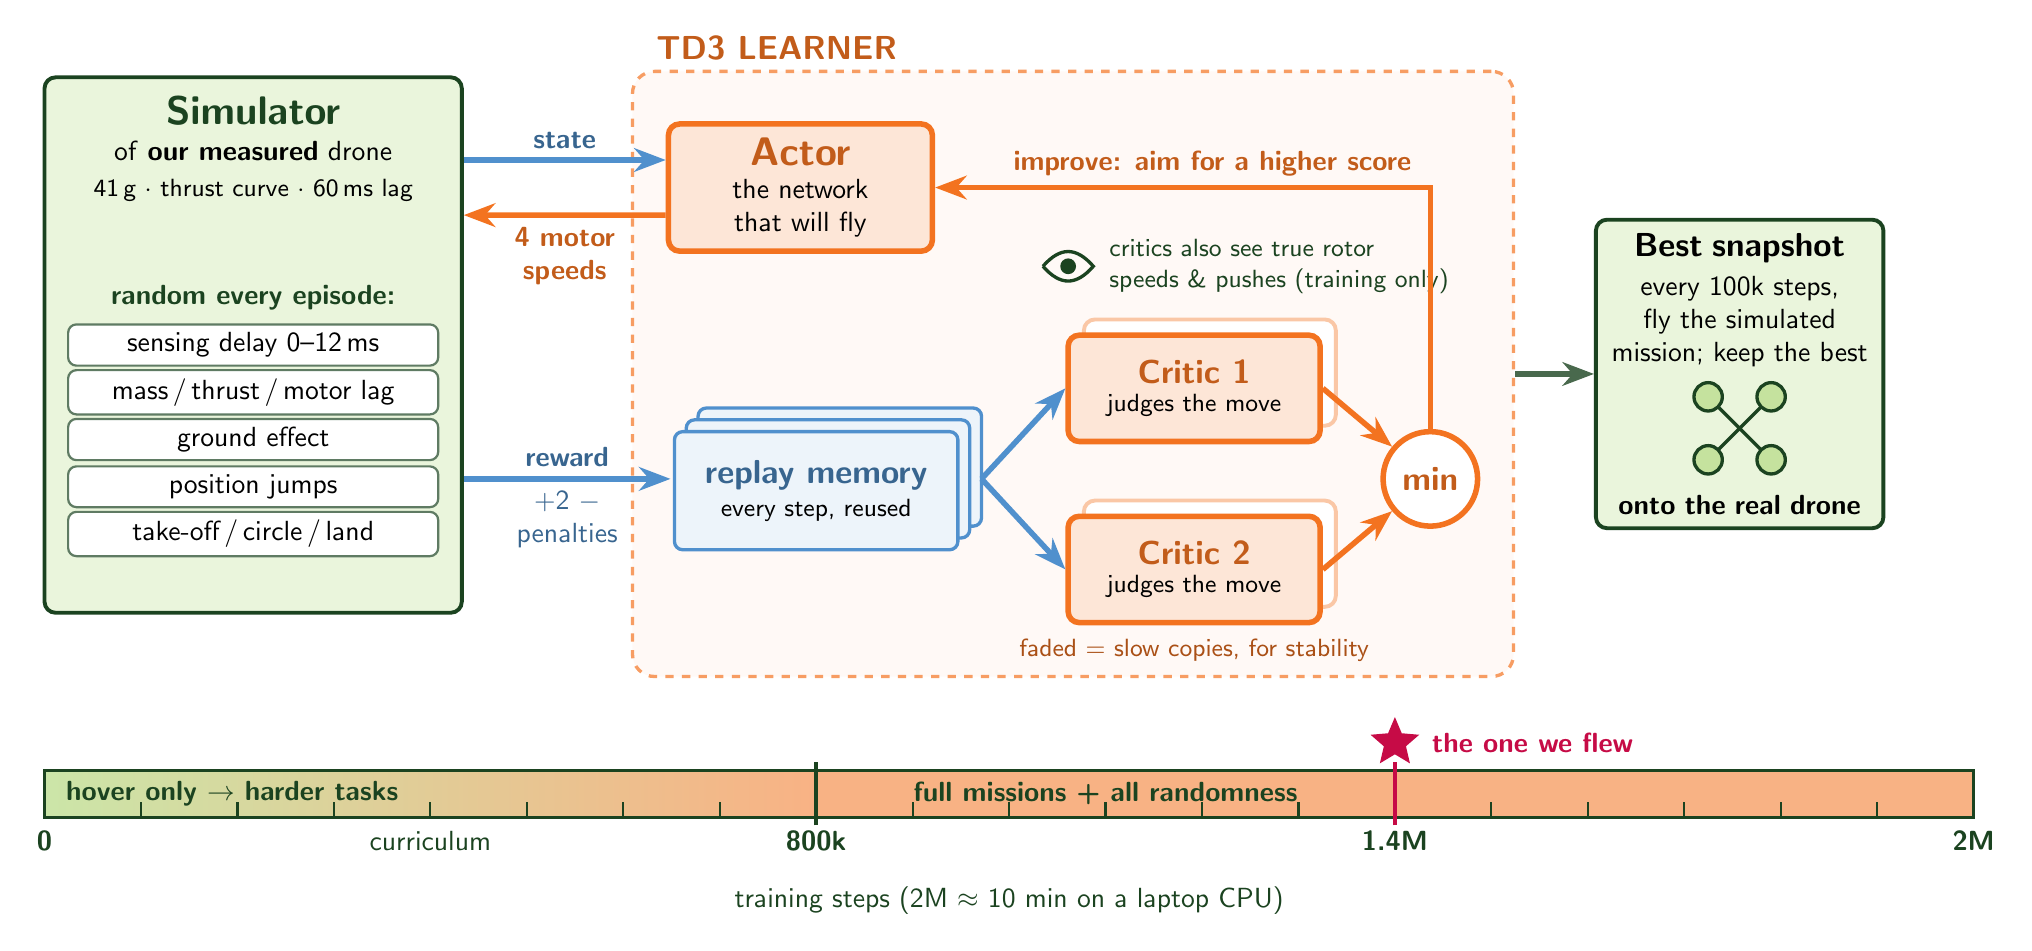
\begin{tikzpicture}
  % ================= simulator =================
  \node[hw, minimum width=5.3cm, minimum height=6.8cm] (sim) at (2.65,0) {};
  \node[anchor=north, align=center] at ($(sim.north)+(0,-0.15)$)
       {{\Large\bfseries\color{saclaydk} Simulator}\\[1pt]{\normalsize of \textbf{our measured} drone}\\[1pt]
        {\small 41\,g $\cdot$ thrust curve $\cdot$ 60\,ms lag}};
  \node[font=\normalsize\bfseries, text=saclaydk] at (2.65,0.6) {random every episode:};
  \foreach \t [count=\k] in {sensing delay 0--12\,ms, mass\,/\,thrust\,/\,motor lag, ground effect, position jumps, take-off\,/\,circle\,/\,land}
    \node[chip] at (2.65, 0.6-\k*0.6) {\t};

  % ================= TD3 learner =================
  \node[nn, text width=3.0cm] (act) at (9.6,2.0)
       {{\Large\bfseries\color{mandarine!80!black} Actor}\\{\normalsize the network\\that will fly}};

  % replay memory: a stack of cards
  \foreach \d in {0.3,0.15,0}
    \draw[draw=bleu, fill=bleu!10, rounded corners=3pt, line width=1.2pt]
      (8.0+\d,-2.6+\d) rectangle (11.6+\d,-1.1+\d);
  \node[align=center] (rep) at (9.8,-1.85) {{\large\bfseries\color{bleu!70!black} replay memory}\\{\small every step, reused}};
  \coordinate (repE) at (11.9,-1.7);
  \coordinate (repSW) at (8.0,-2.6);

  % critics, each with a faded "slow copy" behind it
  \foreach \y/\n in {-0.55/1, -2.85/2} {
    \node[box, draw=mandarine!40, fill=white, minimum width=3.2cm, minimum height=1.35cm]
      at (14.6+0.2, \y+0.2) {};
    \node[nn, minimum width=3.2cm, minimum height=1.35cm] (c\n) at (14.6,\y)
      {{\large\bfseries\color{mandarine!80!black} Critic \n}\\[-2pt]{\small judges the move}};
  }
  \node[font=\small, text=mandarine!70!black, anchor=north] (faded) at ($(c2.south)+(0,-0.05)$) {faded = slow copies, for stability};
  \node[circle, draw=mandarine, fill=white, line width=2pt, font=\large\bfseries, text=mandarine!80!black,
        minimum size=1.2cm, inner sep=0pt] (min) at (17.6,-1.7) {min};

  % eye: critics see extra information
  \begin{scope}[shift={(13.0,1.0)}, line width=1.2pt, draw=saclaydk]
    \draw (-0.32,0) .. controls (-0.1,0.25) and (0.1,0.25) .. (0.32,0) .. controls (0.1,-0.25) and (-0.1,-0.25) .. (-0.32,0);
    \fill[saclaydk] (0,0) circle (0.1);
  \end{scope}
  \node[anchor=west, align=left, font=\small, text=saclaydk] at (13.4,1.0)
       {critics also see true rotor\\speeds \& pushes (training only)};

  % arrows
  \draw[arrb] ($(sim.east)+(0,2.35)$) -- node[above, font=\normalsize\bfseries, text=bleu!70!black] {state} ($(act.west)+(0,0.35)$);
  \draw[arrnn] ($(act.west)+(0,-0.35)$) -- node[below, font=\normalsize\bfseries, text=mandarine!80!black, align=center] {4 motor\\speeds} ($(sim.east)+(0,1.65)$);
  \draw[arrb] ($(sim.east)+(0,-1.7)$) -- node[above, font=\normalsize\bfseries, text=bleu!70!black] {reward}
                                       node[below, font=\normalsize, text=bleu!70!black, align=center] {+2 $-$\\penalties} (7.95,-1.7);
  \draw[arrb] (repE) -- (c1.west);
  \draw[arrb] (repE) -- (c2.west);
  \draw[arrnn] (c1.east) -- (min);
  \draw[arrnn] (c2.east) -- (min);
  \draw[arrnn] (min.north) |- node[pos=0.72, above, font=\normalsize\bfseries, text=mandarine!80!black] {improve: aim for a higher score} (act.east);

  % TD3 zone
  \begin{scope}[on background layer]
    \node[draw=mandarine!70, dashed, line width=1.2pt, rounded corners=8pt, fill=mandarine!4,
          fit=(act)(c1)(c2)(min)(faded)(repSW), inner xsep=12pt, inner ysep=10pt, yshift=8pt] (td3) {};
  \end{scope}
  \node[anchor=south west, font=\large\bfseries, text=mandarine!80!black] at ($(td3.north west)+(0.2,0)$) {TD3 LEARNER};

  % ================= best snapshot to the drone =================
  \node[hw, text width=3.3cm, anchor=west] (best) at ($(td3.east)+(1.0,0)$)
       {{\large\bfseries Best snapshot}\\[2pt]{\normalsize every 100k steps, fly the simulated mission; keep the best}\\[4pt]
        \tikz[line width=1.2pt, saclaydk]{\draw (-0.4,-0.4) -- (0.4,0.4) (-0.4,0.4) -- (0.4,-0.4);
          \foreach \x/\y in {-0.4/-0.4,0.4/0.4,-0.4/0.4,0.4/-0.4} \draw[fill=vert!50] (\x,\y) circle (0.18);}\\[2pt]
        {\normalsize\bfseries onto the real drone}};
  \draw[arr] (td3.east) -- (best.west);

  % ================= training progress bar =================
  \def\bx{0} \def\bw{24.5} \def\by{-6.0}
  \shade[left color=vert!45, right color=mandarine!55] (\bx,\by) rectangle (\bx+0.4*\bw,\by+0.6);
  \fill[mandarine!55] (\bx+0.4*\bw,\by) rectangle (\bx+\bw,\by+0.6);
  \draw[saclaydk, line width=1pt] (\bx,\by) rectangle (\bx+\bw,\by+0.6);
  \foreach \k in {1,...,19} \draw[saclaydk, line width=0.8pt] (\bx+\k*\bw/20,\by) -- ++(0,0.2);
  \draw[saclaydk, line width=1.6pt] (\bx+0.4*\bw,\by-0.1) -- ++(0,0.8);
  \node[anchor=west, font=\normalsize\bfseries, text=saclaydk] at (\bx+0.15,\by+0.3) {hover only $\to$ harder tasks};
  \node[font=\normalsize\bfseries, text=saclaydk] at (\bx+0.55*\bw,\by+0.3) {full missions + all randomness};
  % flown checkpoint marker
  \draw[rouge, line width=1.6pt] (\bx+0.7*\bw,\by-0.1) -- ++(0,0.8);
  \node[star, star points=5, star point ratio=2.2, fill=rouge, inner sep=0pt, minimum size=0.65cm]
    at (\bx+0.7*\bw,\by+0.95) {};
  \node[anchor=west, font=\normalsize\bfseries, text=rouge] at (\bx+0.7*\bw+0.35,\by+0.95) {the one we flew};
  % axis numbers
  \foreach \f/\lab in {0/0, 0.4/800k, 0.7/1.4M, 1/2M}
    \node[anchor=north, font=\normalsize\bfseries, text=saclaydk] at (\bx+\f*\bw,\by-0.05) {\lab};
  \node[anchor=north, font=\normalsize, text=saclaydk] at (\bx+0.2*\bw,\by-0.05) {curriculum};
  \node[anchor=north, font=\normalsize, text=saclaydk] at (\bx+0.5*\bw,\by-0.75) {training steps (2M $\approx$ 10 min on a laptop CPU)};
\end{tikzpicture}
\end{document}
